\documentclass{article}

\usepackage{arxiv}

\usepackage[utf8]{inputenc}
\usepackage[T1]{fontenc}
\usepackage{lmodern}
\usepackage[hidelinks]{hyperref}
\usepackage{url}
\usepackage{booktabs}
\usepackage{amsmath,amssymb,amsfonts,bm}
\usepackage{nicefrac}
\usepackage{microtype}
\usepackage{graphicx}
\usepackage{subcaption}
\usepackage{algorithm}
\usepackage{algpseudocode}
\usepackage{xcolor}
\usepackage{enumitem}
\usepackage[numbers,sort&compress]{natbib}
\setlist{itemsep=1pt,topsep=3pt}
\newcommand{\Ct}{\tilde{C}}

\title{Multi-Agent Compute Scheduling under Congestion}

\renewcommand{\headeright}{Final Project Report}
\renewcommand{\undertitle}{Final Project Report}
\renewcommand{\shorttitle}{Multi-Agent Compute Scheduling under Congestion}

\author{Kshitij Srivastava\\ Roll No.\ 24110174\\ IIT Gandhinagar\\ \texttt{kshitij.srivastava@iitgn.ac.in}
\And Kushal Kumar\\ Roll No.\ 24110178\\ IIT Gandhinagar\\ \texttt{24110178@iitgn.ac.in}
\AND Vishawraj Meena\\ Roll No.\ 24110388\\ IIT Gandhinagar\\ \texttt{24110388@iitgn.ac.in}
\And Tejas Prasad\\ Roll No.\ 23110369\\ IIT Gandhinagar\\ \texttt{tejas.prasad@iitgn.ac.in}}
\date{}

\begin{document}
\maketitle

\begin{abstract}
$N$ users submit jobs to $K$ heterogeneous compute servers, and a resource manager
distributes a limited budget of extra capacity among the servers to reduce congestion.
We formulate the manager's problem as a Markov decision process (MDP) over discretised
server-congestion levels, complete the transition model and termination rule left open
in the proposal, and build a simulator in which users schedule themselves randomly,
selfishly (Nash equilibrium of a congestion game) or cooperatively (social optimum).
We train a tabular Q-learning manager and compare it with model-based dynamic
programming (DP) and four baselines. With random users, Q-learning gives the best cost of all implementable
managers (71.5\% below no allocation, 21.8\% below a uniform split). With strategic users
(selfish or cooperative), Q-learning and DP stay within 4--11\% of a simple threshold
heuristic, because the coarse 27-state observation hides the backlog and demand
information they would need to do better. Selfish routing costs only about 7\% more delay
than cooperative routing (empirical price of anarchy 1.07).
\end{abstract}

\keywords{Congestion games \and Price of anarchy \and Markov decision processes \and Q-learning \and Dynamic programming \and Resource allocation}

%=====================================================================
\section{Introduction}
When many jobs are sent to the same server, queues grow and every user waits longer.
In our setting $N$ users each choose one of $K$ servers, and a resource manager can
temporarily add up to $B$ units of capacity per time step (e.g.\ spare cores or
cloud bursts). Extra capacity reduces delay but is costly, so the manager must decide
\emph{where} and \emph{how much} to allocate using only coarse congestion observations.
Because users react to capacity (selfish users move towards boosted servers), the
manager is effectively playing against a population of strategic agents.

Resource allocation games study agents that compete for limited resources and whose
decisions influence one another~\cite{avni2020dynamic}, and coordination between the
decisions of different users or machines is a central issue in
scheduling~\cite{lee2012coordination}. Multi-agent reinforcement learning has also been
applied to resource allocation in computing and communication systems~\cite{liu2020marl}.
Users choosing among shared servers form a congestion game, which always has a pure Nash
equilibrium~\cite{rosenthal1973}. Selfish choices are generally not socially optimal; the
ratio between the two is the price of anarchy~\cite{koutsoupias1999}, which has been
studied extensively for selfish routing~\cite{roughgarden2002}. The manager's sequential
decision problem is naturally an MDP~\cite{puterman1994}, which can be solved by dynamic
programming when the model is known~\cite{bellman1957} or learned from interaction with
Q-learning~\cite{watkins1992,sutton2018} when it is not.

Our main research question, as stated in the proposal, is: \emph{how do selfish and
cooperative scheduling behaviours differ under congestion, and can adaptive resource
allocation reduce the resulting inefficiency?}

Our contributions are: (i)~a fully specified MDP, including an explicit workload/backlog
transition model and a finite-horizon termination rule (Section~\ref{sec:mdp});
(ii)~an open-source simulator with three user scheduling models
(Section~\ref{sec:method}); (iii)~Q-learning and DP managers evaluated against
baselines and an oracle, with sweeps over the cost weight $\lambda$, the budget $B$ and
the learning rate (Section~\ref{sec:results}).

%=====================================================================
\section{Preliminaries}\label{sec:prelim}

\paragraph{Notation.} Table~\ref{tab:notation} lists the symbols used throughout.
\begin{table}[h]
\centering\small
\begin{tabular}{@{}ll@{\hspace{2em}}ll@{}}
\toprule
$N$, $K$ & number of users, servers & $L_i$ & workload of user $i$\\
$a_i\in\{1,\dots,K\}$ & server chosen by user $i$ & $C_j$ & base capacity of server $j$\\
$b_j$ & backlog carried by server $j$ & $W_j$ & total work at server $j$\\
$d_j$ & extra units given to server $j$ & $\eta$ & capacity per extra unit\\
$B$ & budget (units per step) & $\Ct_j=C_j+\eta d_j$ & effective capacity\\
$\kappa$ & delay exponent & $\lambda$ & cost per resource unit\\
$\tau_1<\tau_2$ & congestion thresholds & $T$, $\gamma$ & horizon, discount factor\\
\bottomrule
\end{tabular}
\caption{Notation.}
\label{tab:notation}
\end{table}

\paragraph{Markov decision process.} An MDP is a tuple $(\mathcal S,\mathcal A,P,R,\gamma)$
with states $\mathcal S$, actions $\mathcal A$, transition probabilities
$P(s'\mid s,a)$, reward $R(s,a)$ and discount $\gamma\in[0,1)$~\cite{puterman1994}.
A policy $\pi$ maps states to actions. Its action-value function
$Q^\pi(s,a)=\mathbb E_\pi\!\left[\sum_{t}\gamma^tR_t\mid s_0=s,a_0=a\right]$ is the expected
discounted return. The optimal values satisfy the Bellman optimality equation
\begin{equation}
Q^*(s,a)=R(s,a)+\gamma\sum_{s'}P(s'\mid s,a)\max_{a'}Q^*(s',a'),
\label{eq:bellman}
\end{equation}
and $V^*(s)=\max_aQ^*(s,a)$~\cite{bellman1957}. Value iteration applies
\eqref{eq:bellman} repeatedly when $P$ and $R$ are known; Q-learning estimates $Q^*$
from sampled transitions without a model~\cite{watkins1992,sutton2018}.

\paragraph{Congestion game and Nash equilibrium.} Each user $i$ picks a server $a_i$ and
pays a cost that grows with the total work on that server. An assignment
$\bm a$ is a \emph{pure Nash equilibrium} if no user can lower its own cost by changing
server while the others stay put. Congestion games always have such an equilibrium, and
best-response dynamics reach one~\cite{rosenthal1973}.

\paragraph{Social cost and price of anarchy.} The social cost of an assignment is the
total delay of all users, $SC(\bm a)=\sum_iD_{a_i}(\bm a)$. The social optimum minimises
$SC$, and the \emph{price of anarchy} is
$\mathrm{PoA}=SC(\bm a^{\text{NE}})/SC(\bm a^{\text{OPT}})\ge1$~\cite{koutsoupias1999,roughgarden2002}.
We report an empirical PoA: the average delay under selfish routing divided by that under
cooperative routing.

%=====================================================================
\section{Problem Formulation (MDP)}\label{sec:mdp}
The manager's problem is the MDP $\mathcal{M}=(\mathcal{S},\mathcal{D},P,R,\gamma)$.

\paragraph{Loads.} $W_j(\bm a)=b_j+\sum_{i}L_i\,\mathbb 1(a_i=j)$ and
$\Ct_j=C_j+\eta d_j$.

\paragraph{State.} The manager observes the normalised load $z_j=W_j/C_j$ \emph{before}
allocating, discretised with thresholds $\tau_1<\tau_2$ into
$x_j\in\{0,1,2\}$ (low / moderate / high). The state is
$\bm x=(x_1,\dots,x_K)\in\mathcal S=\{0,1,2\}^K$, so $|\mathcal S|=3^K$.

\paragraph{Actions.}
$\mathcal D=\{\bm d\in\mathbb Z_{\ge0}^K:\sum_j d_j\le B\}$; unused budget is allowed.
For $K=3,B=4$, $|\mathcal D|=\binom{B+K}{K}=35$.

\paragraph{Reward.} With delay $D_j=(W_j/\Ct_j)^{\kappa}$ ($\kappa\ge1$) experienced by
every user on server $j$,
\begin{equation}
R(\bm x,\bm d)=-\sum_{i=1}^{N}D_{a_i}(\bm a,\bm d)-\lambda\sum_{j=1}^{K}d_j .
\label{eq:reward}
\end{equation}

\paragraph{Transition model.} $P(\bm x'\mid\bm x,\bm d)$ is defined by the simulator
dynamics of Section~\ref{sec:env}: served work is $\Ct_j$, leftover work becomes next
step's backlog, new workloads come from a hidden two-regime demand process, and users
re-select servers after seeing the capacities produced by $\bm d$. Hence $\bm d$
influences the next state through both the backlog and user behaviour, and the
transition is stochastic.

\paragraph{Termination.} An episode ends after exactly $T$ decisions; we
optimise $J(\pi)=\mathbb E_\pi\!\left[\sum_{t=0}^{T-1}\gamma^tR_t\right]$.

%=====================================================================
\section{Methodology}\label{sec:method}
\subsection{Simulation environment}\label{sec:env}
Each step $t$ proceeds as follows:
\begin{enumerate}
\item \textbf{Demand.} A hidden regime $r_t\in\{\text{low},\text{high}\}$ switches with
probability $p_{\text{sw}}$. Workloads are drawn as
$L_{i,t}=\mu_{r_t}\cdot u_i$, $u_i\sim\mathcal U(0.5,1.5)$.
\item \textbf{User scheduling.} Users pick servers with one of the rules in
Section~\ref{sec:users}, using the capacities $c_j=C_j+\eta d_{j,t-1}$ they saw last step
(the current allocation is not yet known).
\item \textbf{Observation.} The manager observes $\bm x_t$ (discretised $W_j/C_j$).
\item \textbf{Allocation.} The manager chooses $\bm d_t\in\mathcal D$ and receives reward
\eqref{eq:reward}.
\item \textbf{Service.} Each server processes $\Ct_j$ units; the backlog becomes
$b_j\leftarrow\min\{\max(W_j-\Ct_j,0),\,C_j\}$ (work beyond one step of base capacity is
dropped/timed out, which keeps queues bounded).
\end{enumerate}
Because the regime and the exact backlog are hidden behind the 27 discrete states, the
manager faces a partially observed problem; the tabular methods treat it as an MDP over
$\bm x$.

\subsection{User scheduling models}\label{sec:users}
\begin{itemize}
\item \textbf{Random:} $a_i\sim\mathcal U\{1,\dots,K\}$ (no coordination).
\item \textbf{Selfish (game-theoretic):} users play a weighted congestion
game~\cite{rosenthal1973} where user $i$'s cost is $(W_{a_i}/c_{a_i})^\kappa$. We run
asynchronous best-response dynamics (random user order, warm-started from the previous
step's assignment) until no user can improve, i.e.\ a pure Nash equilibrium, capped at
50 rounds.
\item \textbf{Cooperative:} a planner minimises the social cost
$\sum_j n_j (W_j/c_j)^\kappa$ ($n_j$ = users on server $j$) by greedy insertion of jobs in
decreasing size followed by local search over single moves and pairwise swaps.
\end{itemize}
Comparing selfish and cooperative delay gives an empirical price of anarchy
(Section~\ref{sec:prelim}).

\subsection{Q-learning manager}
The tabular agent~\cite{watkins1992} keeps $Q(\bm x,\bm d)$ for all $27\times35$ pairs
and is trained with $\epsilon$-greedy exploration (Algorithm~\ref{alg:q}); $\epsilon$
decays linearly from 1 to 0.05 over the first 60\% of episodes. Ties in $\arg\max$ are
broken at random.
\begin{algorithm}[h]
\caption{Q-learning resource manager}\label{alg:q}
\begin{algorithmic}[1]
\State $Q(\bm x,\bm d)\gets0$ for all $\bm x\in\mathcal S,\bm d\in\mathcal D$
\For{episode $e=1,\dots,E$}
  \State $\bm x_0\gets$ \textsc{Reset}(); $\epsilon\gets\epsilon(e)$
  \For{$t=0,\dots,T-1$}
    \State $\bm d_t\gets$ random action w.p.\ $\epsilon$, else $\arg\max_{\bm d}Q(\bm x_t,\bm d)$
    \State $(\bm x_{t+1},R_t)\gets$ \textsc{Step}$(\bm d_t)$
    \State $y\gets R_t$ if $t=T-1$ else $R_t+\gamma\max_{\bm d'}Q(\bm x_{t+1},\bm d')$
    \State $Q(\bm x_t,\bm d_t)\gets(1-\alpha)Q(\bm x_t,\bm d_t)+\alpha\,y$
  \EndFor
\EndFor
\end{algorithmic}
\end{algorithm}

\subsection{Dynamic programming manager}
DP needs $P$ and $R$, which are not available in closed form. We therefore use
\emph{certainty-equivalent} DP: run uniformly random allocations for $E_{\text{DP}}$
episodes, estimate $\hat P(\bm x'\mid\bm x,\bm d)$ by counts and $\hat R(\bm x,\bm d)$ by
sample means, and solve
$V(\bm x)=\max_{\bm d}\big[\hat R(\bm x,\bm d)+\gamma\sum_{\bm x'}\hat P(\bm x'\mid\bm x,\bm d)V(\bm x')\big]$
by value iteration~\cite{puterman1994} (tolerance $10^{-8}$). Unvisited pairs get a
uniform $\hat P$ and a pessimistic reward (the lowest observed value).

\subsection{Baselines}
\textbf{No allocation} ($\bm d=\bm 0$);
\textbf{Uniform} (always spend $B$ evenly, remainder to the smallest servers);
\textbf{Threshold heuristic} (2 units to each level-2 server, then 1 unit to each level-1
server, smallest capacity first, until the budget is used);
\textbf{Myopic oracle} (sees the \emph{exact} loads rather than $\bm x$ and picks the action
maximising the immediate reward; a strong reference that is not implementable from the
state alone).

\subsection{Experimental setup}
Table~\ref{tab:setup} lists the parameters. Every manager is evaluated greedily on the
same 200 held-out episodes (common random numbers). Q-learning and DP are trained with
three seeds (0, 1, 2), so their reported means cover 600 episodes (3 seeds $\times$ 200);
the baselines are deterministic and are evaluated once on the same 200 episodes. All
means are given $\pm$ a 95\% confidence interval. The main metric is the discounted return
$J(\pi)$. We also report the average total user delay per step (equal to $N\cdot D_{\mathrm{avg}}$,
where $D_{\mathrm{avg}}$ is the average delay per user defined in the proposal) and the
number of resource units used per step.
\paragraph{Changes from the proposal.} (i)~The user utility
$U_i=V_i-\beta_iD_{a_i}-c_{a_i}$ was simplified to pure delay ($V_i=0$, $\beta_i=1$,
$c_j=0$), so selfish users minimise their own delay and total welfare equals minus the
total delay. (ii)~The congestion-greedy allocation became the threshold heuristic above,
which also gives units to the most congested servers first. (iii)~The true transition
model $P$ has no closed form, so DP uses an estimated model (certainty-equivalent DP)
instead of serving as an exact benchmark; the myopic oracle, which sees exact loads, is
used as the reference policy instead of $\mathrm{Gap}(\pi)$.

\begin{table}[h]
\centering\small
\begin{tabular}{@{}ll@{\hspace{2em}}ll@{}}
\toprule
Users $N$ / servers $K$ & 12 / 3 & Base capacities $\bm C$ & (4, 6, 10)\\
Capacity per unit $\eta$ & 2 & Budget $B$ & 4 ($|\mathcal D|=35$)\\
Delay exponent $\kappa$ & 2 & Resource cost $\lambda$ & 1\\
Thresholds $(\tau_1,\tau_2)$ & (0.75, 1.25) & Mean job size (low / high) & 1.2 / 2.2\\
Regime switch prob.\ $p_{\text{sw}}$ & 0.1 & Horizon $T$ / discount $\gamma$ & 50 / 0.95\\
Q-learning episodes & 10{,}000 & $\epsilon$ schedule & $1\to0.05$ (first 60\%)\\
Learning rate & $\alpha=\max(0.01,\,n(\bm x,\bm d)^{-0.6})$ & DP exploration episodes & 1{,}500\\
\bottomrule
\end{tabular}
\caption{Default experimental parameters (sweeps vary one parameter at a time).}
\label{tab:setup}
\end{table}
The visit-count learning rate satisfies the Robbins--Monro conditions; polynomial rates
of this form are analysed in~\cite{evendar2003}. We chose it after a constant
$\alpha=0.1$ with 3{,}000 episodes did worse than the heuristics; the sensitivity study in
Section~\ref{sec:alpha} compares both.

%=====================================================================
\section{Results}\label{sec:results}
\subsection{Learning behaviour}
Figure~\ref{fig:curves} shows the training return. In all three user models the return
improves steadily while $\epsilon$ decays and levels off after about 6{,}000 episodes, once
exploration reaches its floor. Averaged over seeds, the 200-episode return improves from
$-607$ to $-315$ with random users, from $-401$ to $-242$ with selfish users, and from
$-365$ to $-242$ with cooperative users. The shaded bands (standard deviation over seeds)
are narrow, so training is stable. Value iteration for DP converged in about 400 sweeps.
The random-exploration data covered 83--95\% of the $945$ state--action pairs.

\begin{figure}[h]
\centering
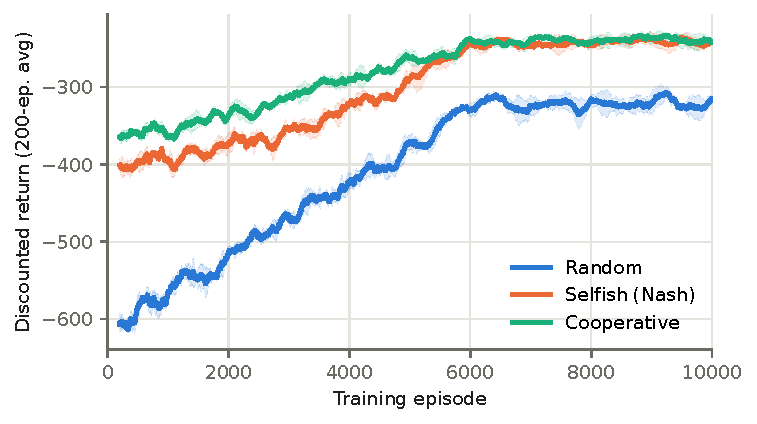
\includegraphics[width=0.72\linewidth]{../results/figures/learning_curves.pdf}
\caption{Q-learning training return (200-episode moving average; band = $\pm1$ s.d.\ over
3 seeds). Training returns include $\epsilon$-greedy exploration.}
\label{fig:curves}
\end{figure}

\subsection{Comparison of resource managers}
Table~\ref{tab:main} and Figure~\ref{fig:cmp} compare all managers.

\begin{table}[h]
\centering\small
\begin{tabular}{@{}lccc@{}}
\toprule
Manager & Discounted return $J$ ($\uparrow$) & Delay / step ($\downarrow$) & Units / step\\
\midrule
\textit{Random users} & & &\\
\quad No alloc. & -1042.8 $\pm$ 39.2 & 57.73 & 0.00\\
\quad Uniform & -380.1 $\pm$ 13.7 & 16.76 & 4.00\\
\quad Threshold & -312.9 $\pm$ 11.1 & 13.99 & 3.03\\
\quad DP & -299.6 $\pm$ 5.9 & 12.67 & 3.62\\
\quad Q-learning & \textbf{-297.1 $\pm$ 5.6} & 12.41 & 3.75\\
\quad Myopic oracle & -267.6 $\pm$ 9.1 & 11.20 & 3.42\\
\midrule
\textit{Selfish (Nash) users} & & &\\
\quad No alloc. & -576.0 $\pm$ 31.6 & 32.68 & 0.00\\
\quad Uniform & -209.2 $\pm$ 5.1 & 7.29 & 4.00\\
\quad Threshold & \textbf{-200.8 $\pm$ 5.7} & 8.26 & 2.57\\
\quad DP & -223.2 $\pm$ 4.0 & 8.68 & 3.29\\
\quad Q-learning & -220.4 $\pm$ 3.3 & 8.48 & 3.43\\
\quad Myopic oracle & -199.0 $\pm$ 5.3 & 8.23 & 2.53\\
\midrule
\textit{Cooperative users} & & &\\
\quad No alloc. & -547.4 $\pm$ 33.5 & 30.63 & 0.00\\
\quad Uniform & -207.2 $\pm$ 5.5 & 7.14 & 4.00\\
\quad Threshold & \textbf{-202.0 $\pm$ 6.3} & 8.10 & 2.70\\
\quad DP & -210.7 $\pm$ 3.6 & 7.77 & 3.52\\
\quad Q-learning & -217.6 $\pm$ 3.6 & 8.19 & 3.42\\
\quad Myopic oracle & -195.3 $\pm$ 6.0 & 8.24 & 2.29\\
\bottomrule

\end{tabular}
\caption{Evaluation results ($\pm$ 95\% CI). Q-learning and DP: 600 episodes (3 seeds
$\times$ 200); baselines are deterministic and use the same 200 episodes. Bold: best
implementable manager (the myopic oracle sees exact loads and serves only as a reference).}
\label{tab:main}
\end{table}

\begin{figure}[h]
\centering
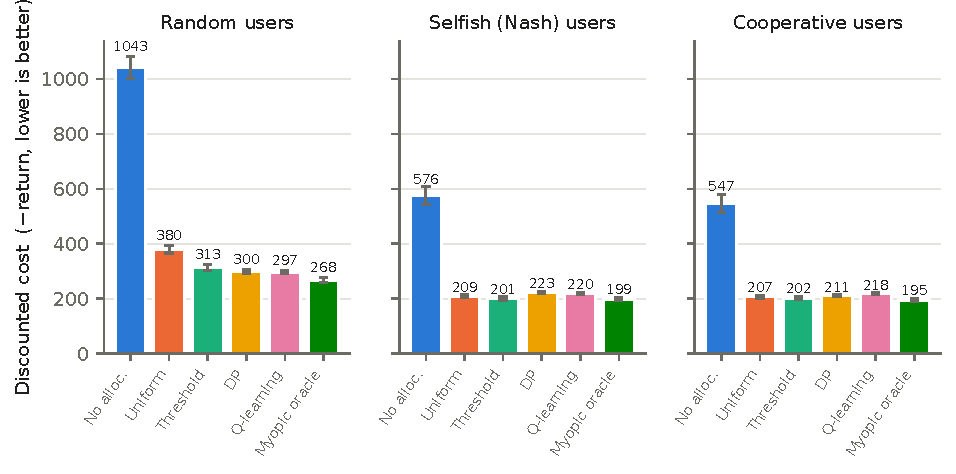
\includegraphics[width=\linewidth]{../results/figures/comparison.pdf}
\caption{Discounted cost ($-J$, lower is better) of every manager under each user model.}
\label{fig:cmp}
\end{figure}

\begin{itemize}
\item \textbf{Allocating capacity matters.} With no allocation, backlogs build up and the
cost is 2.6--3.5 times higher than with any reasonable manager.
\item \textbf{Random users:} Q-learning ($-297.1$) is the best implementable manager. It
beats DP ($-299.6$, within the CI), the threshold rule ($-312.9$, 5.0\% better) and uniform
allocation ($-380.1$, 21.8\% better), and it is 11\% worse than the full-information myopic
oracle. Random routing leaves large, persistent imbalances, so learning where congestion
tends to stay pays off.
\item \textbf{Selfish and cooperative users:} the threshold heuristic is best ($-200.8$ and
$-202.0$), almost matching the oracle. Q-learning is 9.8\% (selfish) and 7.7\%
(cooperative) worse, and DP is 11.2\% and 4.3\% worse. Strategic users already balance
load, so most states look like ``every server is busy''. The remaining differences
depend on the exact backlog and the hidden demand regime, which the 27 discrete states
cannot show. Both learned managers also spend more resources (about 3.4 units per step
versus 2.6 for the threshold rule). Under state aliasing, over-provisioning is the
safe choice.
\item \textbf{Q-learning vs.\ DP} perform similarly (difference within 3.5\%). DP needs far
less data (1{,}500 random episodes versus 10{,}000 learning episodes) but relies on an
estimated model. It is better for cooperative users and slightly worse for selfish users,
where the users' response to the previous allocation makes $\hat P$ less accurate.
\end{itemize}

\subsection{Effect of user behaviour (price of anarchy)}
Figure~\ref{fig:poa} compares per-step delay across user models. Without allocation, the
selfish Nash routing has delay 32.68 against 30.63 for the cooperative optimum, an
empirical price of anarchy of $1.07$. Random routing is $1.88\times$ worse. With a manager
the gap shrinks further, to $1.02$ (threshold) and $1.04$ (Q-learning): extra capacity
absorbs most of the inefficiency of selfish behaviour. In this congestion game,
coordinating the users is therefore much less valuable than coordinating the capacity.
This is consistent with the known result that selfish routing is often close to optimal
in congestion settings~\cite{roughgarden2002}.

\begin{figure}[h]
\centering
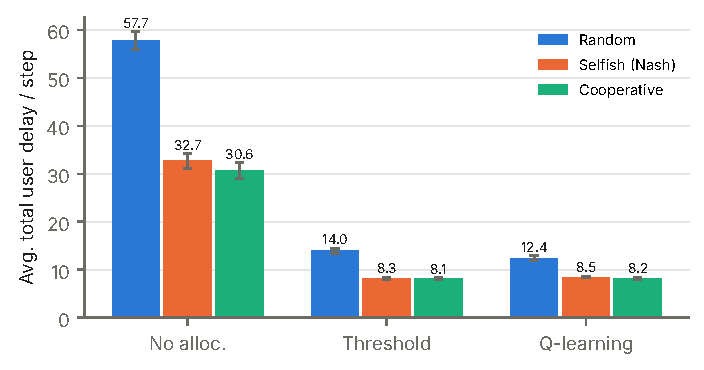
\includegraphics[width=0.66\linewidth]{../results/figures/user_policies.pdf}
\caption{Average total user delay per step for each user model under three managers.}
\label{fig:poa}
\end{figure}

\subsection{\texorpdfstring{Delay--resource trade-off ($\lambda$)}{Delay-resource trade-off (lambda)}}
Figure~\ref{fig:lam} retrains Q-learning (selfish users, 3{,}000 episodes, 3 seeds) for
$\lambda\in\{0,\dots,8\}$. When resources are free ($\lambda=0$) the agent uses 3.72 of the
4 units and reaches the lowest delay (8.48). For $\lambda$ between 0.25 and 4, usage stays
around 3.3 units: congestion relief still outweighs the cost. At $\lambda=8$ usage falls to
2.17 units and delay rises by 89\% to 16.0. $\lambda$ therefore acts as the intended knob,
but the response is close to a step: the marginal delay saved by a unit at a congested
server is large, so the agent only cuts spending once $\lambda$ is very high.

\begin{figure}[h]
\centering
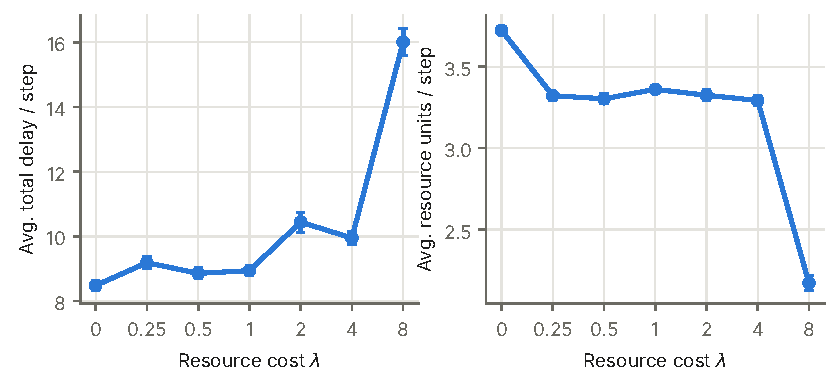
\includegraphics[width=0.8\linewidth]{../results/figures/lambda_sweep.pdf}
\caption{Effect of the resource cost $\lambda$ on delay (left) and resources used (right).}
\label{fig:lam}
\end{figure}

\subsection{\texorpdfstring{Effect of the budget $B$}{Effect of the budget B}}
Figure~\ref{fig:budget} varies $B$ (selfish users). The cost drops steeply up to $B=4$
(Q-learning: $576\to226$, $-61\%$), with diminishing returns after that. Q-learning matches
the threshold rule for $B\le1$ but falls behind as $B$ grows (9.5\% worse at $B=2$). At
$B=6$ its cost even rises slightly ($241.6$), because the action space grows from 35 to 84
actions ($2{,}268$ state--action pairs), which 3{,}000 training episodes cannot cover.
Tabular Q-learning scales poorly with the action space.

\begin{figure}[h]
\centering
\begin{minipage}{0.55\linewidth}\centering
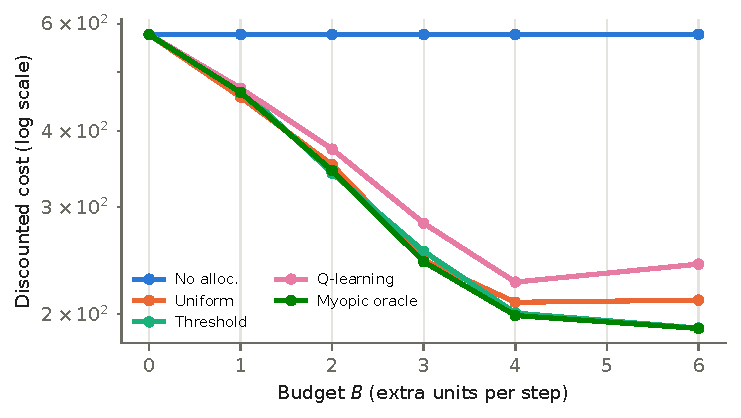
\includegraphics[width=\linewidth]{../results/figures/budget_sweep.pdf}
\caption{Discounted cost vs.\ budget $B$ (log scale).}
\label{fig:budget}
\end{minipage}\hfill
\begin{minipage}{0.42\linewidth}\centering
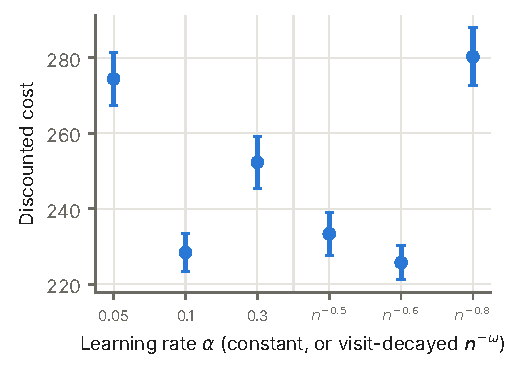
\includegraphics[width=\linewidth]{../results/figures/alpha_sweep.pdf}
\caption{Learning-rate sensitivity (3{,}000 episodes).}
\label{fig:alpha}
\end{minipage}
\end{figure}

\subsection{Learning-rate sensitivity and learned policy}\label{sec:alpha}
Figure~\ref{fig:alpha} compares learning rates (selfish users, 3{,}000 episodes). The
visit-decayed $n^{-0.6}$ is best ($-225.7$), slightly ahead of a constant $0.1$
($-228.4$). Learning rates that are too small ($0.05$) or decay too fast ($n^{-0.8}$) learn
too slowly ($-274$ and $-280$), and a large constant $0.3$ is noisy ($-252$).

Table~\ref{tab:policy} lists the greedy actions for the most visited states. Both
learners send capacity to the small, congested servers. In the most common state
$(2,2,2)$, both choose $(2,2,0)$: the large server (capacity 10) gains the least from
$\eta=2$ extra capacity. The two methods agree on the two most visited states. In lightly
loaded states their choices differ, because almost any allocation clears the congestion
there, so the value differences between actions are small and noisy.

\begin{table}[h]
\centering\small
\begin{tabular}{@{}cccc@{}}
\toprule
State $\bm x$ & Visits & Q-learning $\bm d$ & DP $\bm d$\\
\midrule
(2,2,2) & 60058 & (2,2,0) & (2,2,0)\\
(2,1,1) & 46173 & (4,0,0) & (4,0,0)\\
(0,1,0) & 45906 & (1,2,1) & (3,1,0)\\
(1,0,0) & 44404 & (2,0,1) & (2,0,0)\\
(2,2,1) & 42690 & (2,2,0) & (4,0,0)\\
(0,0,1) & 33053 & (0,3,1) & (2,0,0)\\
(1,1,0) & 28773 & (3,1,0) & (3,0,0)\\
(1,2,1) & 28680 & (0,4,0) & (0,3,0)\\
\bottomrule

\end{tabular}
\caption{Greedy actions in the 8 most visited states (selfish users, seed 0).}
\label{tab:policy}
\end{table}

\subsection{Discussion and limitations}
The main limitation is the \emph{state abstraction}. Three congestion levels per server
hide the backlog size and the demand regime, so the problem is really partially observed.
A hand-designed rule that encodes ``boost the small busy servers'' is already near-optimal
for balanced (strategic) traffic. Learning helps most when the traffic pattern is
persistent and uninformed (random users). Natural extensions are a finer state
(including the previous allocation and backlog bins), function approximation (DQN) to
handle larger $K$ and $B$, and modelling users that also learn, which turns the problem
into a Stackelberg/multi-agent RL problem.

%=====================================================================
\section{Contribution}
\begin{center}\small
\begin{tabular}{@{}p{2.9cm}p{8.6cm}c@{}}
\toprule
Member & Assigned task (from proposal) and delivered work & Fulfilled\\
\midrule
Kshitij Srivastava & Game-theoretic formulation and selfish scheduling model: congestion-game
cost, best-response dynamics to a Nash equilibrium (\texttt{scheduling.py}), price-of-anarchy
analysis. & Yes\\
Kushal Kumar & Cooperative scheduling formulation and overall problem setup: MDP
specification, completed transition model and termination rule, simulator
(\texttt{env.py}), social-optimum planner. & Yes\\
Vishawraj Meena & Q-learning and dynamic-programming implementation: tabular Q-learning,
certainty-equivalent DP / value iteration, baselines (\texttt{agents.py}). & Yes\\
Tejas Prasad & Experimental design, evaluation metrics and parameter analysis: evaluation
protocol, $\lambda$/$B$/$\alpha$ sweeps, figures and tables (\texttt{experiments/}). & Yes\\
\bottomrule
\end{tabular}
\end{center}
\vspace{-0.6em}
\noindent All members contributed to the implementation, the experiments, the discussion
of results and the preparation of this report.

%=====================================================================
\section{Conclusion}
We fully specified the congestion-control MDP, including the transition model and the
termination rule, and built a simulator with random, selfish and cooperative users.
Tabular Q-learning and model-based DP both learn sensible allocation policies that cut
cost by 60--72\% relative to no allocation. Q-learning is the best implementable manager
when users route randomly. With strategic users, a simple threshold rule remains
competitive, because coarse congestion levels hide the information needed to do
better. Selfish routing turned out to be nearly efficient (price of anarchy $\approx1.07$),
and capacity allocation reduces the remaining gap further.

\paragraph{Code and reproducibility.} All results in this report are produced by
\texttt{experiments/run\_all.py} followed by \texttt{experiments/make\_figures.py}
(fixed seeds) in our repository: \url{https://github.com/kus-coded/compute-scheduling-rl}.

\begin{thebibliography}{9}
\bibitem[Rosenthal(1973)]{rosenthal1973}
R.~W. Rosenthal.
\newblock A class of games possessing pure-strategy {N}ash equilibria.
\newblock \emph{International Journal of Game Theory}, 2(1):65--67, 1973.

\bibitem[Koutsoupias and Papadimitriou(1999)]{koutsoupias1999}
E.~Koutsoupias and C.~Papadimitriou.
\newblock Worst-case equilibria.
\newblock In \emph{Proc.\ 16th Annual Symposium on Theoretical Aspects of Computer
  Science (STACS)}, LNCS 1563, pages 404--413. Springer, 1999.

\bibitem[Roughgarden and Tardos(2002)]{roughgarden2002}
T.~Roughgarden and {\'E}.~Tardos.
\newblock How bad is selfish routing?
\newblock \emph{Journal of the ACM}, 49(2):236--259, 2002.

\bibitem[Avni et~al.(2020)]{avni2020dynamic}
G.~Avni, T.~A. Henzinger, and O.~Kupferman.
\newblock Dynamic resource allocation games.
\newblock \emph{Theoretical Computer Science}, 807:42--55, 2020.

\bibitem[Lee et~al.(2012)]{lee2012coordination}
K.~Lee, J.~Y.-T. Leung, and M.~Pinedo.
\newblock Coordination mechanisms for parallel machine scheduling.
\newblock \emph{European Journal of Operational Research}, 220(2):305--313, 2012.

\bibitem[Liu et~al.(2020)]{liu2020marl}
X.~Liu, J.~Yu, and Y.~Gao.
\newblock Multi-agent reinforcement learning for resource allocation in {IoT} networks
  with edge computing.
\newblock arXiv:2004.02315, 2020.

\bibitem[Bellman(1957)]{bellman1957}
R.~Bellman.
\newblock \emph{Dynamic Programming}.
\newblock Princeton University Press, 1957.

\bibitem[Puterman(1994)]{puterman1994}
M.~L. Puterman.
\newblock \emph{Markov Decision Processes: Discrete Stochastic Dynamic Programming}.
\newblock Wiley, 1994.

\bibitem[Watkins and Dayan(1992)]{watkins1992}
C.~J. C.~H. Watkins and P.~Dayan.
\newblock Q-learning.
\newblock \emph{Machine Learning}, 8(3--4):279--292, 1992.

\bibitem[Sutton and Barto(2018)]{sutton2018}
R.~S. Sutton and A.~G. Barto.
\newblock \emph{Reinforcement Learning: An Introduction}.
\newblock MIT Press, 2nd edition, 2018.

\bibitem[Even-Dar and Mansour(2003)]{evendar2003}
E.~Even-Dar and Y.~Mansour.
\newblock Learning rates for {Q}-learning.
\newblock \emph{Journal of Machine Learning Research}, 5:1--25, 2003.
\end{thebibliography}

\end{document}
